\documentclass{article}
\usepackage[a4paper, tmargin=1in, bmargin=1in]{geometry}
\usepackage[utf8]{inputenc}
\usepackage{graphicx}
\usepackage{mathtools}
\usepackage{pdflscape}
\usepackage{listings}
\usepackage{hyperref}
\usepackage{caption}
\usepackage{subcaption}
\usepackage{amsfonts}


\title{CS 754 : Advanced Image Processing Assignment 2}
\author{Sudeep Salgia - 14D070011\\
  Parth Kothari - 14D070019\\
}
\date{\today}

\begin{document}
\maketitle

\section*{Q1}

The given question involves the estimation of $x \in \mathbb{R}^n , n >> 2 $ from a vector $y \in \mathbb{R}^m , m << n $ from measurements of the form $ y = \Phi x $ where $ \Phi $ is called the sensing or measurement matrix and is completely known to us.

\subsection*{A1.a}

It is given that $ x $ has exactly one non-zero element. Now, in the case we have only one measurement i.e., $ m = 1 $, we cannot determine the vector $ x $ from this measurememt. This is because, the value of $y = \Phi x $ is a real scalar which could expressed as a product of two real numbers in infinite ways. Say $ \Phi = [ \phi_1 \ \phi_2 \ \dots \phi_n] $ and $ x = [x_1 \  x_2 \ \dots \ x_n]^T $ and let $ x_k \neq 0 $. Thus, we can write, $ y = \phi_k x_k $, and it is impossible to determine the value of $ k $ just given the value of $y$ and $\phi_i 's$ because $ \forall \ i \ \exists \ x_i $ such that $ y = \phi_i x_i $. This is assuming the no element in the measurement matrix is zero. Even if it were, then we would be certain of the index of the non zero element but not its value. However, in general it is not possible. \\

However, if we knew the index of the non-zero element we can determine the value of unknown vector $x$. This is because we would exactly know the value with which we have mutliplied the non zero value in the vector $x$ because we know all the elements of the measurement matrix. Say the index was $p$, the vector $x$ would have $0$ entries everywhere except at index $p$ where the value would be $\dfrac{y}{\phi_p} $. It is important to note that we ensure that none of the elements in the measurement matrix are zero so that we can ensure the correct retrival of the vector $x$.

\subsection*{A1.b}

The vector $x$ has exactly one non-zero element and we have been given two measurements of that vector, i.e., $ m =2$. Thus, $ y \in \mathbb{R}^{2 \times 1} $ and $ \Phi = [ \phi_1 \ \phi_2 \ \dots \phi_n] $ where $ \phi_i \in \mathbb{R}^{2 \times 1} \forall \ i $. Clearly $y$ lies in the columnspace of the measurement matrix $\Phi$. Since there is exactly one non-zero element in the vector $x$, the vector $y$ would be parallel of one of the columns of the measurement matrix. Now assuming that the measurement matrix has been desgined carefully such that no two columns are parallel, the vector $x$ can be completely reconstructred from the vector $y$ in the following manner. The index of the non zero element, $p$,  can be determined using $ p = \operatorname*{\max}_k \bigg| \dfrac{y^T \phi_k}{\phi_k^T \phi_k} \bigg|$ and the value of the non-zero element is $\dfrac{y^T \phi_p}{\phi_p^T \phi_p} $. However, if the condition of not being parallel is not met, it cannot be guaranteed to uniquely determine $x$ from $y$. If there is exactly one index for which the above expression gets maximised, the above method can be employed. However, in a case where the maximisation expression is maximised for more than one index, we cannot uniquely determine the index of the non-zero element. However the value of the non-zero element can still be determined using the above method using any of the indices for which the expression is maximised upto a sign factor. 


\subsection*{A1.c}

The vector $x$ has exactly two non-zero elements and we have been given three measurements of that vector, i.e., $ m = 3 $. Thus, $ y \in \mathbb{R}^{3 \times 1} $ and $ \Phi = [ \phi_1 \ \phi_2 \ \dots \phi_n] $ where $ \phi_i \in \mathbb{R}^{3 \times 1} \forall \ i $. Again, $y$ lies in the column space of the measurement matrix. However, it is a linear combination of two vectors. It is not always possible to uniquely determine $x$ given $y$, say when the rank of $\Phi$ is $1$ i.e., all the columns are parallel to each other and clearly it is not possible to get a unique solution. We can still uniquely determine $x$ if $\Phi$ obeys certain properties. If the $\phi_i 's$ are such that no three of them are coplanar, then it is definitely possible to uniquely obtain $x$ using the following method. It is important to note that this condition automically ensures no two vectors are parallel. For each unordered pair, $ (\phi_i , \phi_j) $ we can get a vector, $\psi_{ij} $ which is perpendicular to both of them. It is trivial in this case and $\psi_{ij}$ can be easily defined as $ \psi_{ij} = \phi_i \times \phi_j $, i.e., the cross product and then for uniformity, each of them should be normalised. A vector $\psi_{ij}$ is obtained for each pair $ (\phi_i , \phi_j) $. Given the condition assumed on $\Phi$, a vector $\psi_{ij}$ can uniquely determine the pair $ (\phi_i , \phi_j) $. Let the indices at which $x$ is non-zero be $p$ and $q$ and the values there be $\alpha$ and $\beta$ coresspondingly. For all the vectors $\psi_{ij},\  y^T \psi_{ij}$ is computed. Given the assumptions on $\Phi$, there would be exactly one $\psi_{ij}$ for which it is zero, because only the perpendicular vector to $y$ has a zero component along it, which in our case would be $\psi_{pq}$. After that, $\alpha$ and $\beta$ can be unqiuely determined using 
$$ \begin{bmatrix} \alpha \\  \beta \\ \end {bmatrix} = \begin{bmatrix} \phi_p^T \phi_p & \phi_p^T \phi_q \\ \phi_q^T \phi_p & \phi_q^T \phi_q \\ \end{bmatrix}^{-1} \begin{bmatrix} \phi_p^T y \\ \phi_q^T y \\ \end{bmatrix} $$ 

If $\Phi$ does not obey this property, there is no guarantee that this approach will work.
	






% The output is denoised very nicely. However the image has become a little blur during this denoising.

% \begin{figure}[h]
% 	\centering
% 	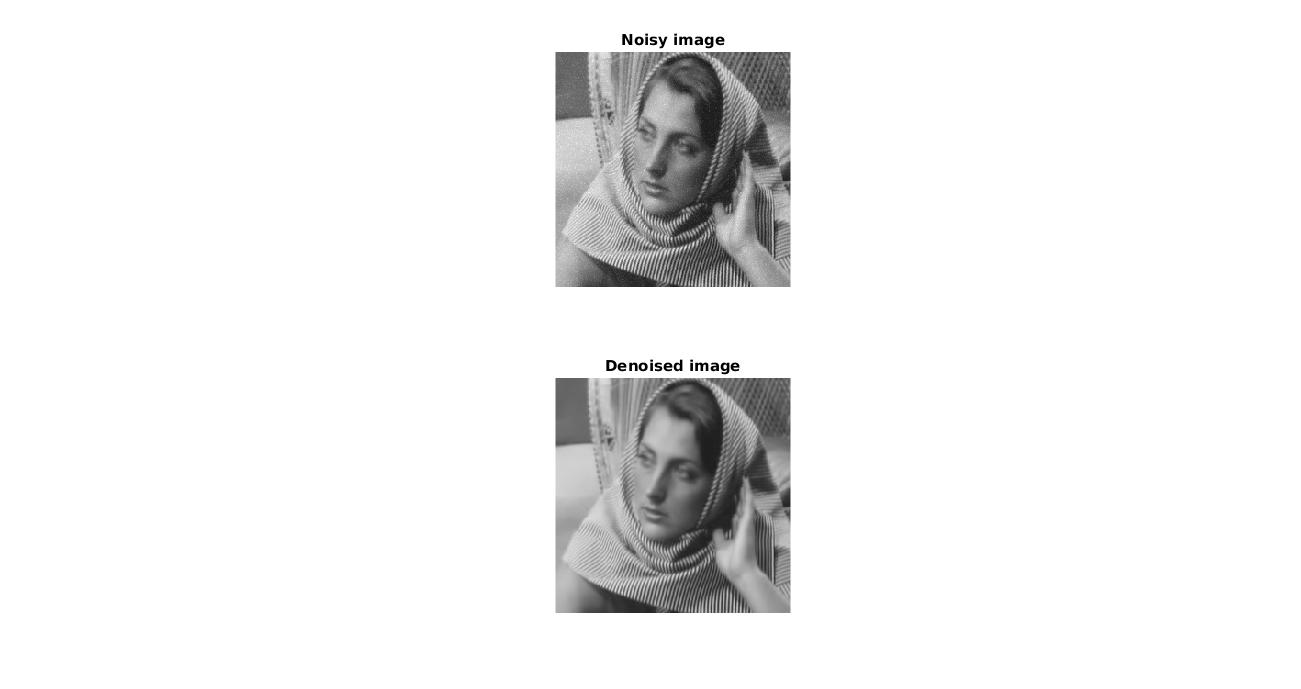
\includegraphics[scale=0.5]{q1a.jpg}
% 	\caption{Question 1a results}
% 	\label{Fig :1a}
% \end{figure}

% \begin{figure}[h]
%   % \centering
%   \begin{subfigure}[t]{0.32\textwidth}
%     \centering
%     \includegraphics[scale=0.5]{images/original_image_barbara}
%     \caption{Original Image Barbara}
%     \label{Fig :1a}
%   \end{subfigure}
%   ~
%   \begin{subfigure}[t]{0.32\textwidth}
%     \centering
%     \includegraphics[scale=0.5]{images/noisy_image_barbara}
%     \caption{Noisy Image Barbara}
%     \label{Fig :1b}
%   \end{subfigure}
%   ~
%   \begin{subfigure}[t]{0.32\textwidth}
%     \centering
%     \includegraphics[scale=0.5]{images/denoised_image_barbara}
%     \caption{Denoised Image Barbara}
%     \label{Fig: 1c}
%   \end{subfigure}

%   \caption{Figures for Q1}
% \end{figure}

\subsection*{A1.d}

This is again an overdetermined system of equations. The vector $x$ has exactly two non-zero elements and we have been given four measurements of that vector, i.e., $ m = 4 $. Thus, $ y \in \mathbb{R}^{4 \times 1} $ and $ \Phi = [ \phi_1 \ \phi_2 \ \dots \phi_n] $ where $ \phi_i \in \mathbb{R}^{4 \times 1} \forall \ i $. Again, $y$ lies in the column space of the measurement matrix and it is a linear combination of two vectors. Now again for solution to exist there must be a condition like similar to the previous question to ensure uniqueness of solution and ability to be determined as well. It turns out that we again we need to enforce that no three vectors are coplanar. However this condition here would be reframed as having that no three vectors have exactly the same two degrees of freedom i.e., correspondng vectors in the basis. So we need to find the pair of vectors from the set $n$ vectors which exactly share the same basis of degrees of freedom as the vector $y$ which is basically solving the system $y = [\phi_i | \phi_j] [\alpha | \beta]$ This will have a solution if the degrees of freedom of $y$ and the vectors $\phi_i$ and $\phi_j$ are the same and also corresponding. And given our assumption, there wil be exactly one such pair. This can be ensured by simple methods like gaussian elimination. And once the condition of the gaussian elimination is satified the other elements will become zero (both in $[\phi_i |\phi_j]$ and $y$ and they would be corresponding ones) and and the system will become a simple set of $2$ linear equations which can be solved by inverting the resultant $2 \times 2$ matrix which is guaranteed to have a solution because our initial assumption also ensures that no two vectors can be parallel. With this solution we would not only get the indices of the non zero elements,$(p,q)$ from the fact that $\phi_p$ and $\phi_q$ are the required vectors but also the values at that two indices by solving the simple $2 \times 2$ system of equations. 


% \begin{figure}[h]
%   \begin{subfigure}[t]{0.5\textwidth}
%     \centering
%     \includegraphics[scale=0.5]{images/original_image_barbara}
%     \caption{Original Image Barbara}
%     \label{Fig :1a}
%   \end{subfigure}
%   ~
%   \begin{subfigure}[t]{0.5\textwidth}
%     \centering
%     \includegraphics[scale=0.5]{images/phi_reconstructed_barbara}
%     \caption{Reconstructed Image Barbara}
%     \label{Fig :1b}
%   \end{subfigure}
%   \caption{Figures for Q2}
% \end{figure}

% \subsection*{A1.3}
% In the folder q1, run the file deblur.m to get the deblurred image.



\section*{Q2}

\subsection*{A2.b}

\begin{figure}
\centering
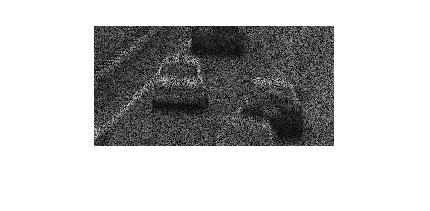
\includegraphics{codedSnapshot}
\caption{Coded Snapshot}
\label{Fig: 2b}
\end{figure}


\subsection*{A2.c}

The given equation is of the form, $$ E(x,y) = \sum_{t} C_t(x,y) \cdot F_t(x,y) $$. We need to convert this into a vectorised form $Ax = b$. Clearly, b is the vectorised form of $E(x,y)$ i.e., $b = \text{vec}(E(x,y))$. Let $f_t = \text{vec}(F_t(x,y))$. To convert the dot product into a matrix-vector form, we need to vectorise one of the matrices and convert the other matrix into a diagonal matrix by first vectorising the matrix and then placing all the elements in the vector formed in as a the diagonal elements of the matrix. Thus we can write $c_t = \text{diag}(C_t)(x,y)$ and therefore we can write, $ C_t(x,y) \cdot F_t(x,y) = c_t f_t $. Now to compute sums of all such vectors we adopt a similiar method. Define $x = [f_1 | f_2 | \dots |f_T ]^T$. Using the same idea of a diagonal matrix we can construct $ A = \text{diag}(c_1, c_2, \dots c_T) $ which means all these matrices are placed along the diagonal of the matrix $A$. Using this construct we can write $Ax = b$ where, $A$, $x$ and $b$ have been defined above.

\subsection*{A2.d}

Using the same principle as above, the vector $b$ is the vectorised version of the corresponding $8 \times 8$ patch on the given snapshot.
Similarly define $C_{t,i}$ and $F_{t,i}$ as the corresponding patches in the code and the image which can be diagonalised and vectorised respectively as before to give $c_{t,i}$ and $f_{t,i}$. Now if $f$ is expressed in some sparse representation in an orthonormal basis, we can write, $f_{t,i} = \Psi \theta_{t,i}$. Thus we have $z = [f_1 | f_2 | \dots |f_T ]^T = [ \Psi \theta_{1,i} | \Psi \theta_{2,i} | \dots | \Psi \theta_{T,i}]^T $ and $ B = \text{diag}(c_1, c_2, \dots c_T) $. The actual product $Bz$ can now be rewritten as $Ax$ where, $ x = [  \theta_{1,i} |  \theta_{2,i} | \dots |  \theta_{T,i}]^T $ and $A = \text{diag}(c_1 \Psi, c_2 \Psi , \dots c_T \Psi) $. Thus using the above definition of $A$, $x$ and $b$, we can write $Ax = b$.

\subsection*{A2.e}

The root mean square error between the original and reconstructed images for $T = 3$ are $0.0752, 0.0954$ and $0.1103$. This is obtained at $\epsilon = 700$. It should be noted that these values change about $\pm 5- 7\%$ for different binary codes.

\subsection*{A2.f}

The root mean square error between the original and reconstructed images for $T = 4$ are $0.1217, 0.1032, 0.9032$ and $0.7906$. This is obtained at $\epsilon = 700$. It should be noted that these values change about $\pm 5- 7\%$ for different binary codes.


\section*{Q3}

We need to prove the bounds on the coherence between the measurement matrix, $\Phi \ \in \ \mathbb{R}^{m \times n}$ and the orthonormal representation matrix $\Psi \ \in \ \mathbb{R}^{n \times n}$ which are given by $(1, \sqrt{n})$. 

\subsection*{A3}

Since $\Psi$ forms an orthonormal basis for vectors in $\mathbb{R}^n$, the rows of the measurement matrix can be expressed in the basis of the representation matrix whose columns are denoted by $\psi_i , \ i = 0,1,2 \dots n $. Let us define $\phi_i^T$ , the $i^{\text{th}}$ row of $\Phi$, as $$ \phi_i = \sum_{k=1}^n \alpha_{ik} \psi_k  \text{; where } \alpha_{ik}   \in  \mathbb{R} \ \forall \ i,k \text{ and } \sum_{k=1}^n \alpha_{ik}^2 = 1 $$ 

Coherence is defined as $ \mu = \sqrt{n} \operatorname*{\max}_{i,j} | \phi_i^T \psi_j | $ which in our context boils down to $\mu = \sqrt{n} \operatorname*{\max}_{i,j} |\alpha_{ij}| $. \\

We will first prove the upper bound. It is clear from the constraint $\sum_{k=1}^n \alpha_{ik}^2 = 1$ that the maximum of $|\alpha_{ik}| = 1$. This is because all the $\alpha_{ik}$'s are real and hence this is the maximum value. And this coherence is the maximum value of the $\alpha_{ik}$ which itself is upper bounded by $1$ and thus the upper bound on coherence is $\sqrt{n}$. \\

For the lower bound, we need to in general consider the following problem  to minimize $ \operatorname*{\max}_{i} |\alpha_i| $ subject to the condition, $\sum_{k=i}^n \alpha_{i}^2 = 1$. Consider the case for $n=2$. The problem is to find the maximum value of function $f(x) = \operatorname*{\min} (x^2, a^2 - x^2) $ where $a$ is a constant. This can be easily solved graphically to obtain that the required answer is $\frac{a}{\sqrt{2}}$. Now consider the case for $n=3$. Fix the value of $\alpha_3$  to be say some real number $b \in (0,1)$. This is now solving a two dimensional problem whose solution we know. And now by varying the value of $b$ we can solve the three dimensional problem which can now be stated a two dimensional problem in the form $f(x) = \operatorname*{\min} (b^2, \frac{1 - b^2}{\sqrt{2}}) $ which again can be solved to obtain the solution $ \frac{1}{\sqrt{3}}$. Thus using a similar argument and induction we can say the solution to our $n$-dimensional problem would be $\frac{1}{\sqrt{n}}$. Consequently the lower bound on coherence will be $1$.


\section*{Q4}


Consider the matrix $A$, the columns of which are unit normalised and the restricted isometry constant (RIC) , $\delta_s$ is given by
$$ (1- \delta_s)||\theta||^2 \leq ||A\theta||^2 \leq (1+\delta_s)||\theta||^2 $$ where $\theta$ is a $s$-sparse vector. 

\subsection*{Q4}

Now, since $\theta$ is a $s$-sparse vector, there are exactly $s$ columns of $A$ that contribute in the product $A\theta$ and hence using only these $s$ columns as support we can write $||A\theta|| = ||A_s \theta_s||$ where $A_s$ is the reduced matrix containing columns only in the support of $\theta$ and similarly we can define $\theta_s$. Thus, we can write, $$ (1- \delta_s)||\theta_s||^2 \leq ||A_s\theta_s||^2 \leq (1+\delta_s)||\theta_s||^2 $$ using the above fact and also that $||\theta|| = ||\theta_s||$. Say $\theta_s$ is unit norm which is a legit assumption to make calculations easy as we can divide all the sides by the squared norm of $\theta_s$. Now the term $$ || A_s \theta_s ||^2 = \theta_s^T A_s^T A_s \theta_s $$ and is maximised if $\theta$ is along the eigen vector of the largest eigen value of $A_s^T A_s$ and similarly minimised for the minimum eigen vector. Say the maximum and minimum eigen values are $\lambda_{\text{max}}$ and $\lambda_{\text{min}}$.  RIC can be alternatively stated as $\max(\lambda_{\text{max}} -1, 1 - \lambda_{\text{min}}) $ Now consider the matrix $C = A_s^T A_s$ and using the definition of coherence $\mu = \operatorname*{\max}_{i,j, i\neq j} |A_i . A_j| $ , we can say that coherence is the upper bound on the magntiude of the off diagonal elements of $C$. Since columns of $A$ were unit normalised so would be those of $A_s$ and the diagonal terms in the matrix $C$ will be $1$. Using the Gershgorin's theorem we can say that at least one eigen value of $C$ lies in a circle centred at $C_{ii}$ and of radius $R_i, \ \forall \ i$. The radius $R_i$ is defined as the sum of the magnitudes of the off diagonal elements in the $i^{\text{th}}$ row. Since the way the matrix $C$ is constructed each of such off diagonal is upper bounded, the radius term is upper bounded by $\mu (s-1)$ since there are $s-1$ off diagonal terms. Here, $C_{ii} = 1 \forall \ i $. Thus for any eigen value of $C, \lambda$, we can write, $ 1-R_i < \lambda < 1 + R_i $. \\ 

Thus we can write, $ \lambda_{\text{max}} - 1 < 1 + R_i -1$ and since $R_i \leq (s-1)\mu$, thus we can write when $\delta_s = \lambda_{\text{max}} -1 $ that $\delta_s \leq \mu (s-1)$.  Similarly for the case when $\delta_s = 1 - \lambda_{\text{min}}$ we can use the fact that $1-R_i < \lambda_{\text{min}} \implies 1 - \lambda_{\text{min}} < 1-1 + R_i$ and using the upper bound on the radius we can again conclude that $\delta_s \leq \mu (s-1)$ which completes the proof.

 




\end{document}

